%%%% Paramétrage du TD %%%%
\def\xxactivite{Colle 04 \ifprof -- Corrigé \else \fi} % \normalsize \vspace{-.4cm}
\def\xxauteur{\textsl{Xavier Pessoles}}


\def\xxnumchapitre{Chapitre 1 \vspace{.2cm}}
\def\xxchapitre{\hspace{.12cm} Correction des systèmes}

\def\xxcompetences{%
\textsl{%
\textbf{Savoirs et compétences :}\\ \vspace{-.4cm}
\begin{itemize}[label=\ding{112},font=\color{ocre}]
\item \textit{C1-02 : }Proposer une démarche de réglage d'un correcteur.
\item \textit{C2-04 : }Mettre en œuvre une démarche de réglage d’un correcteur.
\end{itemize}
}}

\def\xxtitreexo{Réglage d'un correcteur proportionnel et d'un correcteur intégral}
\def\xxsourceexo{\hspace{.2cm} Pôle Chateaubriand -- Joliot Curie}
\def\xxauteur{\textsl{Xavier Pessoles}}

\def\xxfigures{
%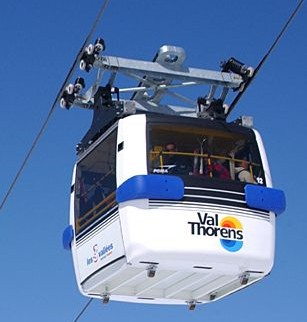
\includegraphics[width=.35\linewidth]{fig_00}
}%figues de la page de garde


\input{\repRel/Style/pagegarde_TD}
\setcounter{numques}{0}


\setlength{\columnseprule}{.1pt}

\pagestyle{fancy}
\thispagestyle{plain}

\vspace{4.9cm}

\def\columnseprulecolor{\color{ocre}}
\setlength{\columnseprule}{0.4pt} 

%%%%%%%%%%%%%%%%%%%%%%%

\setcounter{exo}{0}
\begin{multicols}{2}

\subsection*{Correction proportionnelle}
Soit $F(p)$ la FTBO d'un système bouclé à retour unitaire. Les diagrammes de BODE de $F(p)$ sont représentés
sur la figure ci-dessous.

\question{Déterminer les marges de phase et de gain du système, puis conclure quant à sa stabilité.}


On décide d’ajouter au système un correcteur série de type proportionnel. On note $K_p$ le gain de ce
correcteur.

\question{Déterminer la valeur de $K_p$ permettant d’obtenir une marge de gain $M_G =\SI{12}{dB}$.}

\question{Déterminer la nouvelle marge de phase du système.}

\question{En le justifiant, déterminer l’erreur de position du système corrigé pour une consigne indicielle.}


\subsection*{Correction intégrale -- Asservissement en accélération}
\setcounter{exo}{0}
On désire contrôler l'accélération $\gamma(t)$ d'un plateau. Pour cela, un capteur d'accélération, fixé sur le plateau
et de sensibilité $B$, est utilisé dans la chaîne de retour du système. Le moteur permettant la motorisation du
plateau est modélisé par la fonction de transfert : $H(s)=\dfrac{A}{1+\tau s}$. 
On modélise le correcteur par la fonction de transfert $C(s)$.
\begin{center}
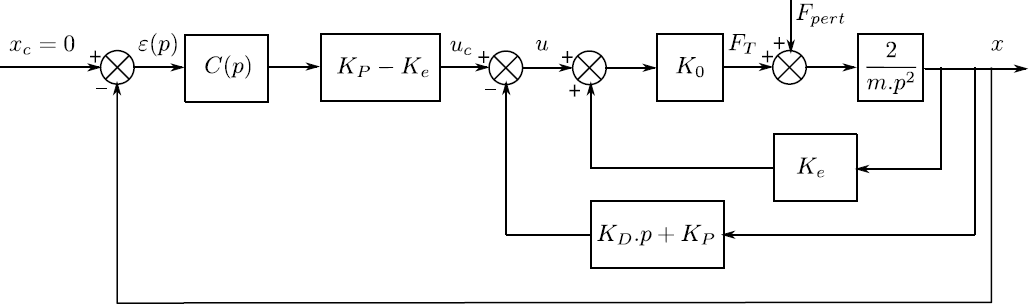
\includegraphics[width=\linewidth]{fig_02}
\end{center}

On a $A=\SI{100}{g.m.s^{-2}.V^{-1}}$, $\tau=\SI{0,2}{s}$ et $B=10^{-2}\,\text{g}^{-1}\text{V}\text{m}^{-1}\text{s}^{-2}$.

\question{Quelle doit être la fonction de transfert du transducteur $T(s)$ qui traduira l’accélération de consigne $\Gamma_c(s)$ en tension $E(s)$.}

On applique à l’entrée du système une consigne d’accélération $\gamma_c=20 g$.

Système asservi sans correction : $C(s)=1$.
\question{Déterminer l'expression de la fonction de transfert en boucle fermée de ce système. Identifier les différents paramètres de cette fonction. Réaliser l'application numérique.}

\question{Calculer le temps de réponse à 5\% de ce système pour une entrée en échelon.}

\question{Donner la valeur de l'accélération en régime permanent. Ce système est-il précis ? Donner l'erreur en régime permanent.}

\question{Donner l'allure de la réponse de ce système en précisant les points caractéristiques.}

Système asservi avec correction intégrale : $C(s)=\dfrac{1}{s}$.

\question{Déterminer l'expression de la fonction de transfert en boucle fermée de ce système. Identifier les
différents paramètres de cette fonction. Réaliser l'application numérique.}

\question{Calculer le temps de réponse à 5\% de ce système pour une entrée en échelon.}

\question{Donner la valeur de l'accélération en régime permanent. Ce système est-il précis ? Donner l'erreur en
régime permanent. Pouvait-on prévoir ce résultat.}

\question{Conclure en comparant le comportement du système avec et sans correction.}

\end{multicols}
\begin{center}
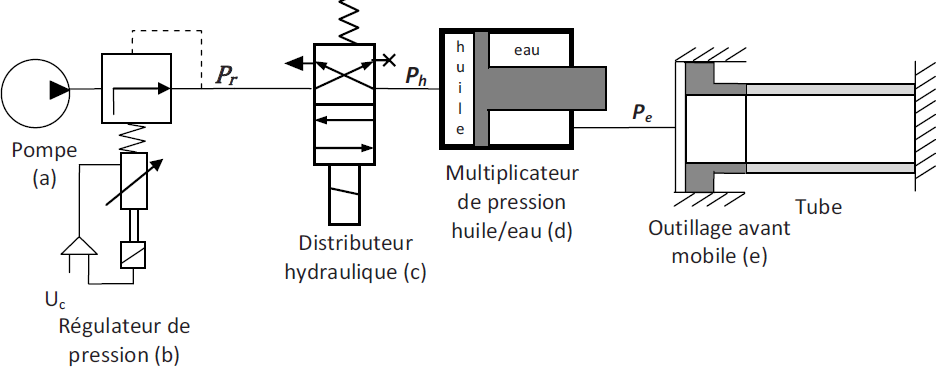
\includegraphics[width=\linewidth]{fig_01}
\end{center}

\ifprof
\newpage
\begin{center}
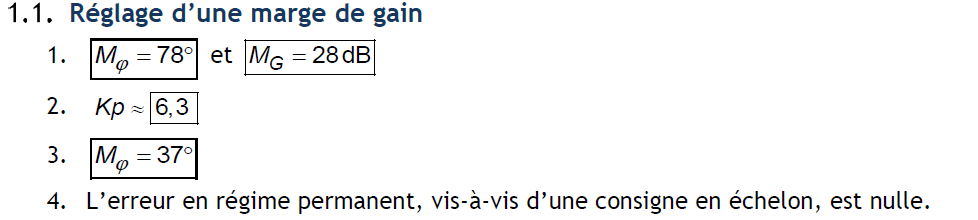
\includegraphics[width=\linewidth]{cor_01}
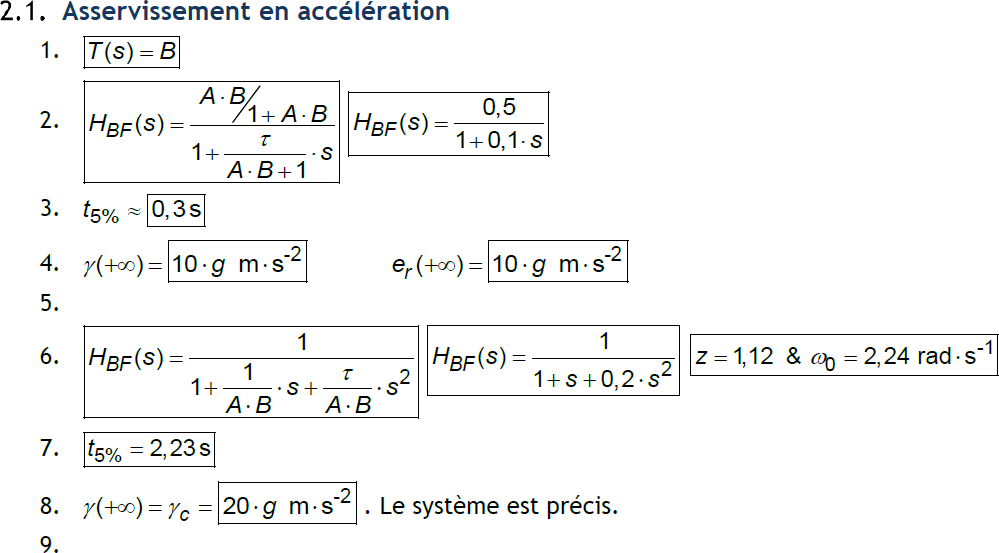
\includegraphics[width=\linewidth]{cor_02}
\end{center}
\else
\fi
